\section{A New Design for Building Secure Virtualization Systems}
\label{sec.design}

This section discusses how to use the observation
 that ``commonly used kernel paths'' contain fewer bugs 
(\S{\ref{sec.metric}}) to build secure virtualization systems.
The key idea of our design is that all code \emph{including the complex part
of the operating system API} should have a very small TCB that accesses only 
commonly used kernel paths. 
Any complex or possibly risky system functions 
are reimplemented by our own code within a sandbox. This makes any bugs or failures within the implementation of those complex system functions 
to be contained by the sandbox. As result untrusted code will not have the possibility to reach 
and trigger sensitive and risky portions of the kernel. 


\begin{figure}%[h]
\centering
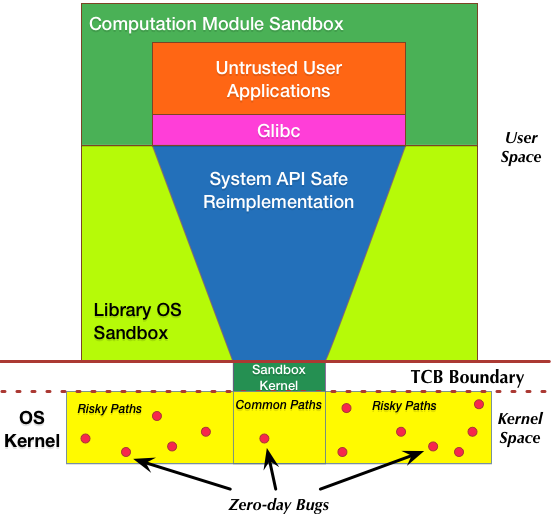
\includegraphics[width=1.0\columnwidth]{diagram/lind_secure_design_new.png}
\caption{``Safe-Reimplementation'' design to ensure predictable execution of untrusted user codes despite existing potential zero-day bugs within the OS kernel.} 
\label{fig:design}
\end{figure}

\subsection{Architecture}

To execute untrusted applications in a safe manner that will not trigger bugs 
in the underlying OS kernel, %and cause damage to other parts of the system, 
we must build a virtualization system that can provide isolation and 
containment for any improper operations in the programs. 
One approach to building such a system is to place it entirely in the user space, 
and to only have a small sandbox kernel with restricted access to the OS kernel (Figure \ref{fig:design}). 
This approach has advantages over other approaches that require modifications to 
the OS kernel, as it avoids the risk of threat escalation. If modified modules 
are inside the OS kernel, they have kernel privileges that could allow attacks on the underlying OS, 
as well as applications run on top of it. 

There are two main components in our design of a secure virtualization system, as shown in Figure \ref{fig:design}. 
The first is a computation module, which performs functions like type checking, object creation, 
and garbage collection. The second is a library OS that serves requests to access the OS kernel. 
Those two components should work together to complete the requirements of running user code. 
To run this code in our virtualization system, we first invoke the computation module to perform its operations. 
Whenever there are system call requests, 
the computation module will direct those requests to our library OS. 
The library OS will respond to the system call requests and return results to the user code if the requests are granted. 

\subsubsection{The Computation Module}

Our secure system should be able to support and run legacy applications, 
and execute binary code compiled from unmodified source code on popular hardware architecture, 
like x86 architecture. Providing an execution environment that can run unmodified source code is 
the main responsibility of the computation module. The key security issue of executing system calls 
without triggering OS kernel bugs is left to the library OS module.

\subsubsection{The Library OS Module}

The Library OS module is the core of our virtualization system. It is comprised of two parts, 
a sandbox kernel that provides access to basic but critical system calls, and a system 
API safe reimplementation that implements more complex calls. 

The sandbox kernel forms the only addition to the TCB of our system.  We 
make this system extremely small and simple so that it is easy to verify its 
security.  The purpose of the sandbox code is simply to provide an API that performs
a few critical system calls with the most basic parameters.  For example,
programs will need some mechanism to write data to the file system
and communicate with the network.  The kernel's goal is to provide the ability
to do so, while utilizing the most simplistic calls possible with the most
basic arguments.  For example, the file system API need only provide a way
to write data to storage.  It need not provide a directory abstraction, the
concept of file permissions, links, or even the concept of multiple files.
It merely needs to provide a mechanism to write out data that can be later
read in.  

%It should have a set of capabilities that enable the construction of essential and more complicated functions. 
%For example, the sandbox kernel capabilities should include basic functions for network, 
%file system I/O, lock, thread, and namespace. It also needs to have access to the OS kernel through system calls. 
%In developing our design, we leveraged our verified hypothesis that commonly used kernel paths contain fewer bugs. 
%Thus, the system calls we allow in our sandbox kernel are common calls, like file open, read, write, and close. 
%Furthermore, the set of arguments used for each call is also highly restricted. 

The system API safe reimplementation is a set of more complicated system calls 
that are constructed from our sandbox kernel. It should be able to reconstruct 
complex system functions, like those complex calls in the file system API. 
We reimplemented those system calls because we did not want user code 
to have direct access to the underlying OS kernel. 
Therefore, our reimplementation layer serves as a mediator between the user code 
and the OS kernel. In our design, the reimplementation is safe 
because the reconstruction of system calls is isolated in a sandbox. 
This can be done by choosing a memory-safe programming language to write code for the reimplementation. 
With this design, even if there are bugs in the function reimplementation, 
they cannot escape from the sandbox and will not reach the underlying OS kernel. 

Here is an example of how this reimplementation would work with the symbolic link function. 
If there is a bug in this function, our safe reimplementation will not rely on the kernel code paths for symbolic links. 
Instead, our sandbox system will implement the incorrect behavior, so the program will not be forced to quit, but will do so in the sandbox. 
Since the reimplementation code does not have privileged access to the system as the OS kernel does, 
this will not result in a security issue. The usual outcome of a bug in this case is simply that the application will fail.

With the computation module and the library OS module, unmodified user code is able to run on top of our designed system. 
It is important to note that our design does not rely on any specific technique or tool. 
To implement the computation module and the library OS module in our design, 
it is possible to choose from several different techniques that fit well with the users' specific needs or requirements.

This general system design was implemented as a prototype called Lind. 
In the next section, we provide a detailed description of Lind.

\subsection{Discussion: Our Design Choice}

In reviewing our design, some fundamental questions could be raised about the dual sandbox design choice. 
Why is one not enough? And, if two is good, why not use three or more? 
The answer to the first question is that the kernel interface is extremely rich and hard to protect. 
In order to have minimal impact on the kernel, as well as provide sufficient API for legacy applications, 
we need to have one sandbox focuses on protecting the kernel and providing POSIX API, 
while a second sandbox focuses on efficiently executing applications. 
So our approach includes two sandboxes, one as the computation module, 
and the other one as library OS module. As to the second question, 
which could be rephrased as ``why not sandbox the sandbox kernel TCB and get more security?,'' 
the lowest level sandbox eventually must have some fundamental, 
even if  limited access to system resources, such as memory, and storage, threads. 
So even if we were to sandbox the sandbox kernel and have additional sandboxes, 
the one at the bottom level will still access the OS kernel in a similar way. 
Thus, having multiple sandboxes does not provide any extra security benefits. 
